\section{Wavelength Division Multiplexing}\label{sec:wdm}
With recent advances in solid state technology, LEDs have emerged as the most energy efficient sources for illumination. SPD of different colored LEDs that emit different narrow-band spectrum can be combined in different ratios to produce different colors for illumination including the shades of white on the black body radiation curve. The ability to combine multiple narrow band sources to generate white light also provides the benefit of being able to transmit concurrent information streams over different color groups; thus enabling WDM. The performance of a multi-colored VLC system depends on a number of parameters including SPD of the transmitting elements, illumination color, filter transmission function, and receiver responsivity.

Lasers and LEDs produce a much smaller SPD width as compared to incandescent and fluorescent sources and are thus preferable for WDM. LED emission can be modeled with a Gaussian distribution as in Eq. (\ref{eqSPDGaussian}) while laser emission can be modeled with a Lorentzian distribution as in Eq. (\ref{eqSPDLorentzian}). Equations in (\ref{eqSPD}) model emission spectra for the $j^{th}$ transmitting element.
\setlength{\arraycolsep}{0.0em}
\begin{subequations}
\begin{align}
S_j(\lambda) &= \frac{1}{\sqrt{2\pi\sigma_j^2}}exp\left[-\frac{(\lambda-\lambda_j)^2}{2\sigma_j^2}\right]\label{eqSPDGaussian}\\
S_j(\lambda) &= \frac{1}{\pi}\frac{0.5\Gamma_j}{(\lambda-\lambda_j)^2 + (0.5\Gamma_j)^2}\label{eqSPDLorentzian}
\end{align}
\label{eqSPD}
\end{subequations}
\setlength{\arraycolsep}{5pt} 
where $\lambda_j$ is the dominant wavelength of emission, $\sigma_j$ is the measure of spread (deviation) from the dominant wavelength for the Gaussian model, and $\Gamma_j$ is the FWHM from the dominant wavelength for the Lorentzian model. At small SPD width, most of the optical power is emitted at the dominant wavelength. At larger SPD widths the optical power is spread across a larger wavelength range and starts overlapping across different transmitting elements, thus causing interference.

To generate white light $W(\lambda)$, emissions from different transmitting elements are weighted by factor $t_j$ before being mixed together. The resulting spectrum is given by
\begin{equation}
	\label{eqWhite}
	W(\lambda) = \sum_{j=1}^{N_{tx}}t_jS_j(\lambda)
\end{equation}

\begin{figure}[!t]
	\centering
		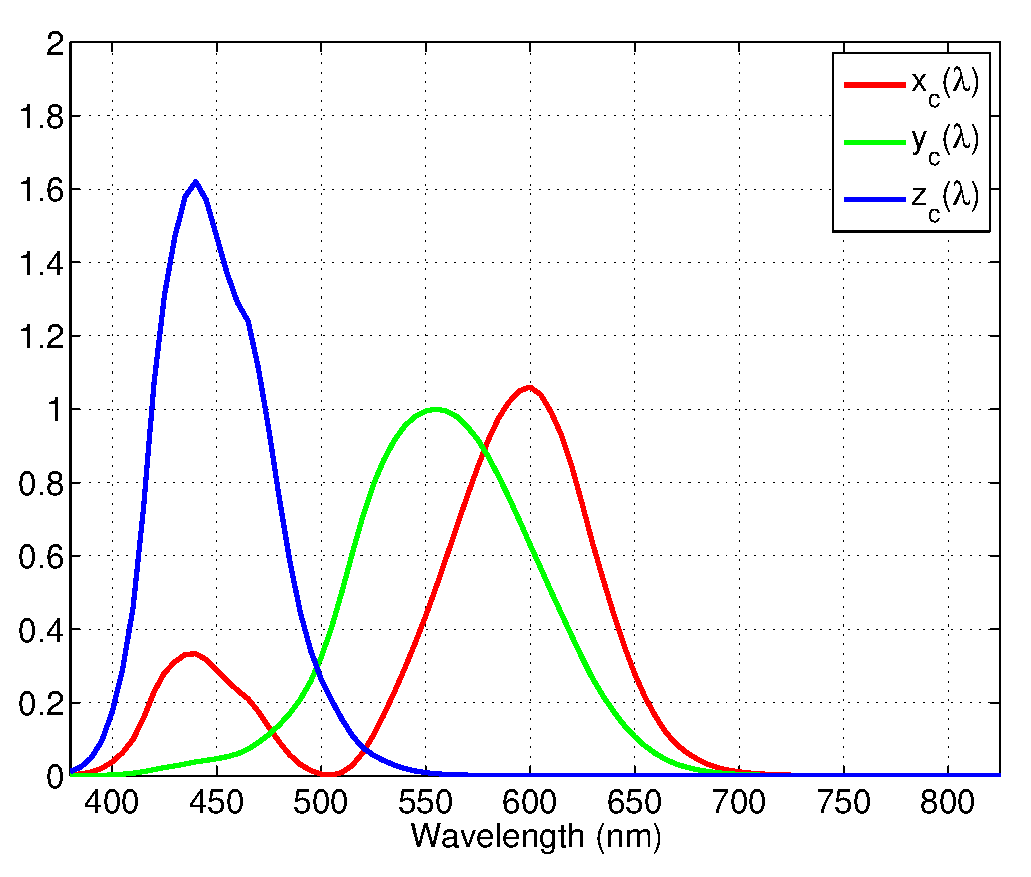
\includegraphics[trim={0.05in 0.05in 0.05in 0.05in}, clip=true, width=2.75in]{img/CIE1931CMF.eps}
	\caption{CIE XYZ 1931 model color matching functions}
	\label{fig:CIE1931CMF}
\end{figure}

The \textit{commission internationale de l'$\acute{e}$clairage} (CIE) specified the CIE 1931 XYZ color space. It maps an SPD to a color representation as sensed by the human eye. The standard defines three color matching functions $x_c(\lambda)$, $y_c(\lambda)$, and $z_c(\lambda)$ as shown in \figurename{ \ref{fig:CIE1931CMF}}. The tristimulus values for the XYZ primaries are given by
\setlength{\arraycolsep}{0.0em}
\begin{subequations}
\begin{align}
X_W &= \int_{\lambda_{min}}^{\lambda_{max}}W(\lambda)x_c(\lambda)d\lambda\\
Y_W &= \int_{\lambda_{min}}^{\lambda_{max}}W(\lambda)y_c(\lambda)d\lambda\\
Z_W &= \int_{\lambda_{min}}^{\lambda_{max}}W(\lambda)z_c(\lambda)d\lambda
\end{align}
\label{eqTriStimulus}
\end{subequations}
\setlength{\arraycolsep}{5pt}

A color can be expressed in terms of its chromaticity and luminance. Chromaticity coordinates capture the hue and saturation of the color while luminance captures the amount of light in the color. The chromaticity coordinates for the SPD can be then be computed from the tristimulus values as
\begin{equation}
\label{eqChromaticity}
	\vecttwo{x}{y} = \frac{1}{X_W+Y_W+Z_W}\vecttwo{X_W}{Y_W}
\end{equation}

The spectral radiance of a black body heated to temperature $T$ as stated by Planck's law is given by
\begin{equation}
\label{eqPlanck}
	 S(\lambda) = \frac{2hc^2}{\lambda^5\left[exp\left(\frac{hc}{\lambda kT}\right)-1\right]}
\end{equation}
where $h$ is the Planck's constant, $c$ is speed of light, and $k$ is Boltzmann's constant. Replacing $W(\lambda)=S(\lambda)$ in Eq.(\ref{eqTriStimulus}) and then from Eq.(\ref{eqChromaticity}) we obtain the CIE 1931 XYZ chromaticity values $[x,y]$ associated with a black body heated to temperature $T$. In this context $T$ is also known as the CCT for color represented by $[x,y]$. Note that two different SPDs can generate the same chromaticity coordinates. This is due to the principle of metamerism.

Traditionally luminaires have been specified to generate a certain CCT with colors at lower temperature appearing (ironically) warm than those at higher temperatures. It is practical to generate colors off the black body radiation curve using different colored lasers and LEDs. However for this analysis, we shall stick to colors generated on the black body radiation curve. As the CCT changes from a lower value to a higher value, the optical power available to transmit information on any color channel varies thus affecting the overall communication performance.

Optical filters can be manufactured to permit narrow bandpass filtering with nanometer precision using plasmonics \cite{xu10a,che12a,yok12a}. Broad bandpass optical filters that make use of interference are widely available. The transmittance of these filters can be modeled as Lorentzian functions of wavelength. The choice of the filter FWHM is a tradeoff to collect the maximum signal while rejecting interference and background illumination.

Responsivity of the receiving elements also affects the aggregate system performance. It depends on the quantum efficiency of the material of sensor. Reference \cite{gha12a} computes responsivity as
\begin{equation}
\label{eqResponsivity}
	 R(\lambda) = \frac{\xi\lambda}{1240}
\end{equation}
where $\xi$ is the quantum efficiency of the material, and $\lambda$ is wavelength of interest. For equal signal radiant flux, signals that span wavelength ranges with lower responsivity will perform poorly as compared to the rest. 
